\chapter{Meglévő megoldásokkal összehasonlítása}

\section{Meglévő ipari megoldások}

\subsection{Schneider Power Monitoring Expert}

\subsubsection{Alapfunkciók}

\begin{itemize}
    \item Segít csökkenteni a meddő teljesítmény termelést és az ebből keletkező büntetéseket.
    \item Saját számlát készít, a helyi mérések alapján, hogy összehasonlítási alap legyen a számlákhoz.
    \item Segít elszámolhatóságot biztosítani alszámlázáshoz.
    \item Berendezések teljesítményét és várható élettartamát ellenőrzi.
    \item Valós idejű adatfigyelés, riasztás és energiafolyamatok vezérlése a létesítményen belül.
    \item Azonosítsa a potenciális áramminőségi problémákat a hálózatában, és értesíti erről a személyzetet.
\end{itemize}
\cite{sePME}

\begin{figure}[ht]
    \centering
    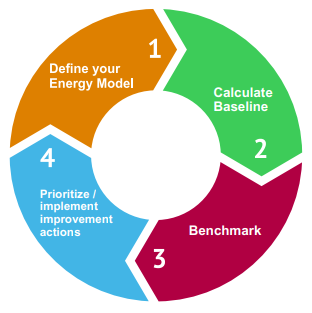
\includegraphics[width=0.3\textwidth]{figures/sePME.png}
    \caption{Schneider Electric PME model\cite{sePME}}
    \label{fig:schneider-pme}
\end{figure}

\subsubsection{Előnyök}

Az energiamérési rendszer használata átlagban 24\%-kal csökkentette a fogyasztást, 
és 30\%-al a költségeket.

Mivel folyamatos megfigyelés és  beavatkozás lehetséges, a problémák korai szakaszában orvosolhatóak így
ezeket 22\%-al lehet csökkenteni. Ez a tudatosság csökkenteni a a hiba utáni visszaállítások idejét is.
Ezenkívül segít a mögöttes problémák megtalálásában is.\cite{sePME}

\subsection{Siemens SIMATIC Energy Suite}

\subsubsection{Alapfunkciók}

A Siemens SIMATIC Energy Management rendszere integrált tehát nem csak megfigyelésre alkalmas hanem vezérlésre is. 
A már létező TIA Portal keretrendszerükbe épül és így egy helyen elérhető a többi rendszerükkel. 
Ez szintén egy moduláris és skálázható rendszer.
Megfelel az ISO 50001 szabványnak, és ez is alkalmazható terhelés figyelésre számlázásra és rendszerelemzésre,
mint az előzőleg taglalt rendszer.\cite{sieEMS}

\subsubsection{Előnyök}

\begin{itemize}
    \item Terepi szintű integráció saját és más eszközökkel. Figyelve itt az egyedi eszközökre.
    \item Gyártás szintű felügyelet. Üzem szintű energia fogyasztást lehet vele figyelni.
    \item Nagyobb rendszerekben vállalati szintű energiaelemzés, ahol több helyszín között is lehet felügyelni.
    \item Ezentúl alkalmas beavatkozásra is. Amennyiben túl nagy a fogyasztás képes fogyasztókat leválasztani távolról is akár.
\end{itemize}
\cite{sieEMS}

\begin{figure}
    \centering
    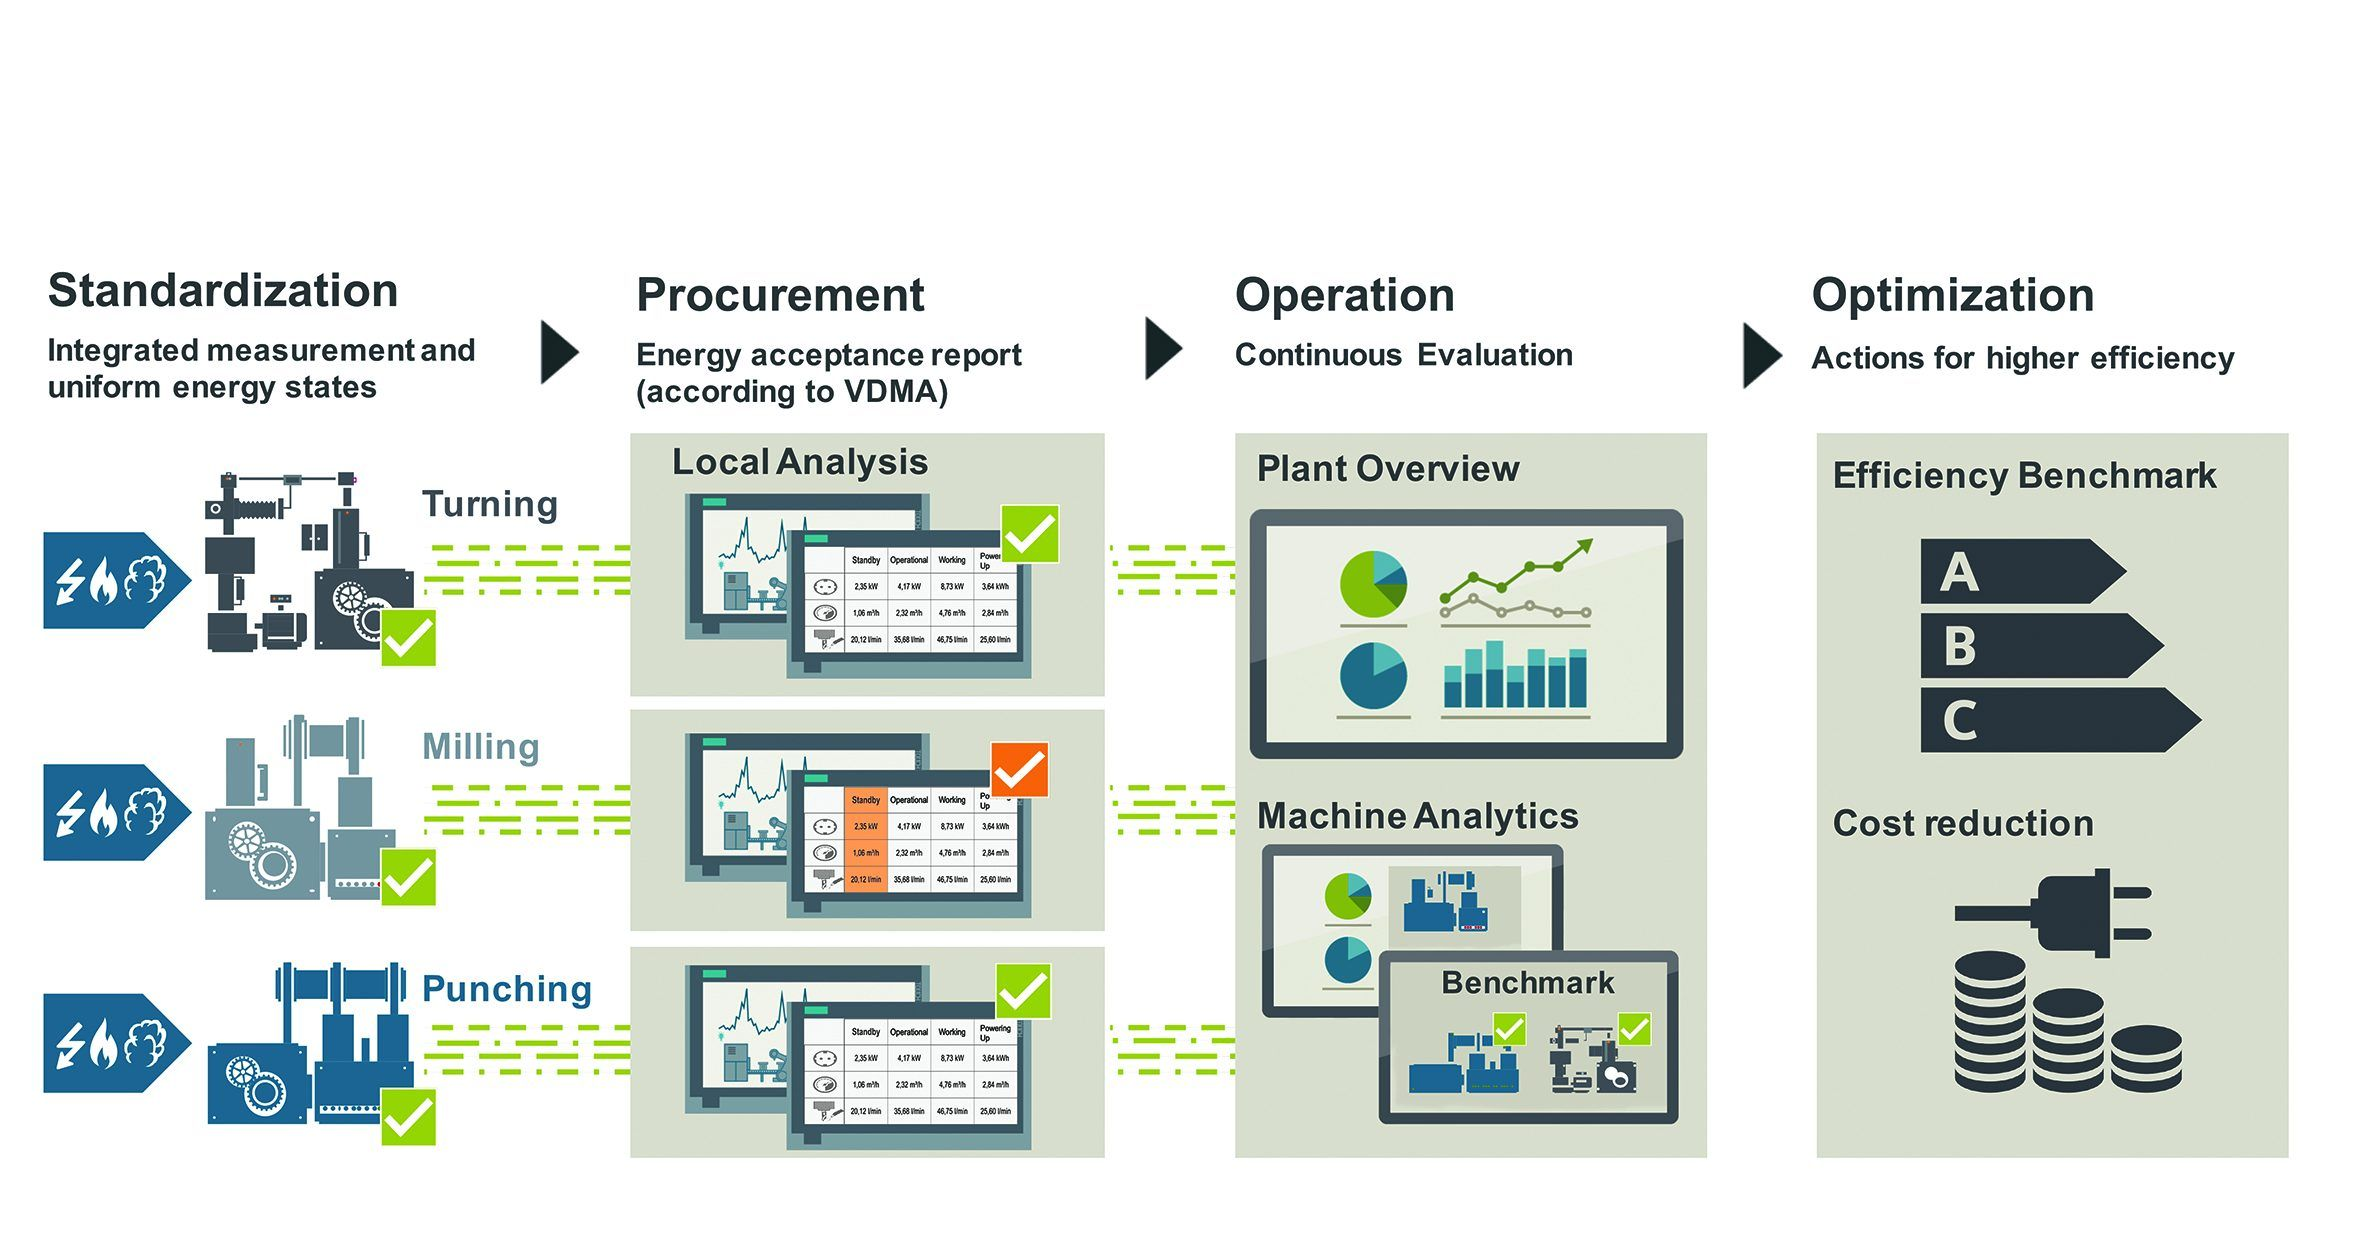
\includegraphics[width=0.8\textwidth]{figures/sieEMS.png}
    \caption{Siemens EMS model\cite{sieEMS}}
    \label{fig:siemens-ems}
\end{figure}

\section{Saját megoldás}

Egy mondatban: a saját eszközkészletem (ESP-8266 + Prometheus + Grafana + Python) 
sokkal  olcsóbb és könyebben módosítható, de a Schneider 
EcoStruxure Power Monitoring Expert (PME) és a Siemens SIMATIC Energy Suite 
olyan pontosságot, energiaminőség-elemzést, ISO-50001-megfelelőséget és 24/7-es 
gyártói támogatást biztosít, aminek megvalósítása nagy munkát és pénzt igényelne.

\newcolumntype{P}[1]{>{\raggedright\arraybackslash}p{#1}}

\begin{table}[ht]
    \centering
    \begin{tabular}{|P{2.5cm}|P{3.5cm}|P{3.5cm}|P{3.5cm}|}
    \hline
    \textbf{Jellemző} & \textbf{Nyílt forráskódú megoldás} & \textbf{Schneider PME} & \textbf{Siemens Energy Suite} \\
    \hline
    Peremi eszközök &
    ESP8266 + CT &
    PowerLogic / ION \& PowerTag mérők, megszakítók, átjárók &
    S7-1500 PLC + Sentron PAC, 7KM PAC, megszakítók \\
    \hline
    Adatátvitel &
    Wi-Fi és HTTPS REST &
    Modbus/TCP &
    PROFINET\\
    \hline
    Adatbázis &
    Prometheus &
    Beépített SQL Express &
    Integrált WinCC SQL archívum \\
    \hline
    Vizualizáció &
    Grafana &
    Webalapú HTML5 irányítópult &
    WinCC HMI képernyő \\
    \hline
    Analitika &
    Ami lekódolásra kerül &
    Harmonikus, villódzás, EN 50160 megfelelés &
    Automatikus terheléskikapcsolás ISO 50001 \\
    \hline
    Licenc költségek &
    Nincs &
    Eszközcsomagok: 5-től korlátlanig; 50-es csomag tízezer eurós nagyságrend &
    Futtatási licenc eszközönként ezer eurós nagyságrend \\
    \hline
    Tipikus ár 50 mérőpontra &
    kb. 1 000 € (panelek + szenzorok + szerver) &
    kb. 10 ezer € (mérők + licenc + szerver) &
    kb. 10 ezer € (mérők, PLC, licencek, TIA Portal) \\
    \hline
    Támogatás &
    Közösségi támogatás; nincs hivatalos tanúsítvány &
    Gyártói 24/7, ISO 50001 &
    Gyártói 24/7, TÜV EN 13849 \\
    \hline
    \end{tabular}\caption{Rendszeráttekintés - összehasonlítás}
    \label{tab:osszehasonlitas}
\end{table}